\documentclass[11pt,a4paper,notitlepage]{article}
\usepackage[margin=3.5cm]{geometry}
\usepackage{amsmath}
\usepackage{amsfonts}
\usepackage{graphicx}
\usepackage[dvipsnames]{xcolor}
\usepackage[most]{tcolorbox}

\tcbset{colback=white!10!white, colframe=black!50!black, 
        highlight math style= {enhanced, %<-- needed for the ’remember’ options
            colframe=red,colback=red!10!white,boxsep=0pt}
        }

\newcommand{\bsym}{\boldsymbol}
\newcommand{\non}{\nonumber}
\newcommand{\nexp}[1]{\text{exp}\left( #1\right)}
\newcommand{\niota}{\dot{\iota}}
\newcommand{\cbrak}[1]{\left( #1 \right)}
\newcommand{\req}[1]{\text{eq}$( #1 )$}
\newcommand{\nsin}[1]{\text{sin}\left( #1 \right)}
\newcommand{\txtgr}[1]{\textcolor{ForestGreen}{#1}}
\newcommand{\txtre}[1]{\textcolor{Red}{#1}}
\newcommand{\todo}{\txtre{[TODO] }}
\newcommand{\done}{\txtgr{[DONE] }}

\begin{document}
\section{Notes of Spherical Ansatz}
\subsection{ED results}
	After establishing that the ansatz we have is the zero-energy eigenstate of model Hamiltonian, we want to check if it produces right excitation properties. First, we checked the density and charge of single quasi-particle and quasi-hole (for $\nu=1/3,2/5$) using exact digonalization: 

	\begin{figure}[h]
		\centering
		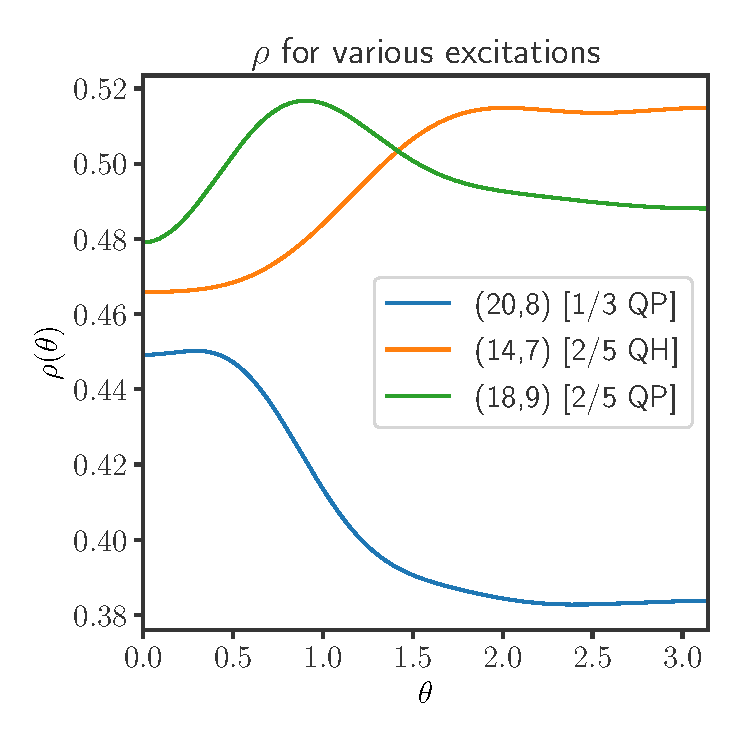
\includegraphics[width=2.5in]{figures/densities_ED.pdf}
		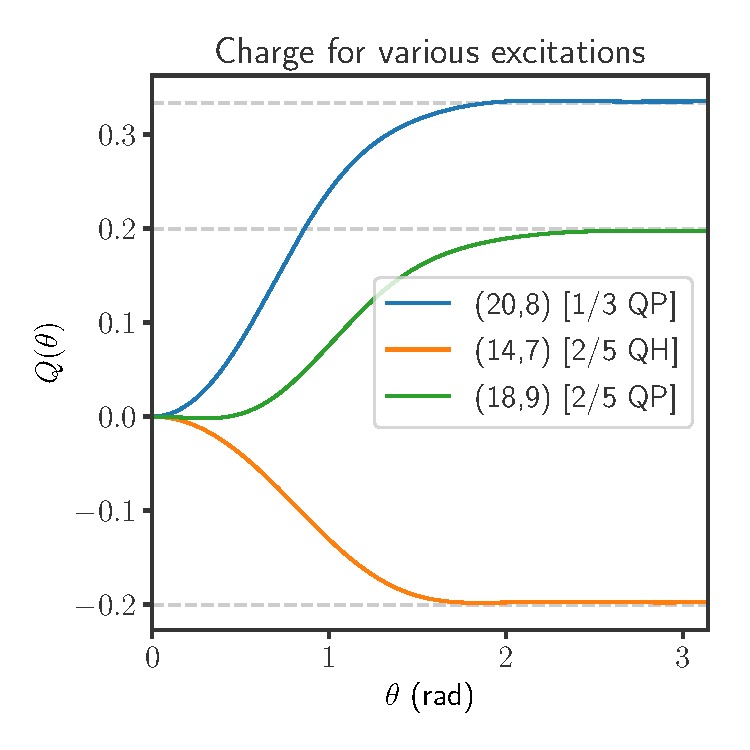
\includegraphics[width=2.5in]{figures/charge_ED.pdf}
		\caption{Density $\rho$ and charge for $2/5$ q-particle and q-hole ($(18,9)$ and $(14,7)$) and $1/3$ q-particle $(20,8)$}
	\end{figure}

	\txtre{NOTE:} In spherical geometry, $\nu=\frac{N}{2Q}$ only when $N\rightarrow \infty$. Hence, instead of getting the right densities, we get a shifted density away from the quasi-particles. For example, in the above figures, $(20,8)$ which is a $1$-qp  system for $\nu=1/3$, we get $\rho=\frac{N-(1/3)}{2Q}\sim 0.3833$ instead of $1/3$.
	
\subsection{Writing ansatz for sphere}
	It produces right density profile and charge for the q-particle and q-holes. This gave us motivation to write the ansatz wavefuntion for spherical-geometry. We tried to do the stereographic projection to get a conversion of coordinates $(x,y)\rightarrow (\theta,\phi)$. We then reached to the following form of wf in spherical geometry :
	
	\begin{align}
		\text{planar }\quad \Psi^{\alpha}_{\nu} &= \prod_{j<k} (\hat{Z}_j-\hat{Z}_k)^{2p}\times \Phi^{\alpha}_{\nu} \\
		\text{spherical }\quad \Psi^{\alpha}_{\nu} &= \Phi^{\alpha}_{\nu}\ (Y_{Q^{*},n,m}\rightarrow (Y_{Q^{*},n,m}-\hat{Y}^{Q-Q^{*}}_{Q^{*},n,m}))\quad \forall n \geq 1
	\end{align}
	
	Where in \req{2}, we replace single particle wf $Y_{Q^{*},n,m}$ with $(Y_{Q^{*},n,m}-\hat{Y}^{Q-Q^{*}}_{Q^{*},n,m})$, where $\hat{Y}^{Q-Q^{*}}_{Q^{*},n,m}$ is an LLL projector type operator $(\text{Jain}, J.15)$ for spherical geometry.\\
	
	 By doing a proportionality check for $1$, $2$ and $3$ quasi-particles with the corresponding ED ground state wf, we have established that this spherical ansatz is equal to ED ground state upto a multiplicative constant. We also reproduce correct charges for $1$ and $2$ q-particles for $\nu=1/3$ using the spherical ansatz.
	 
	 \begin{figure}[h]
		\centering
		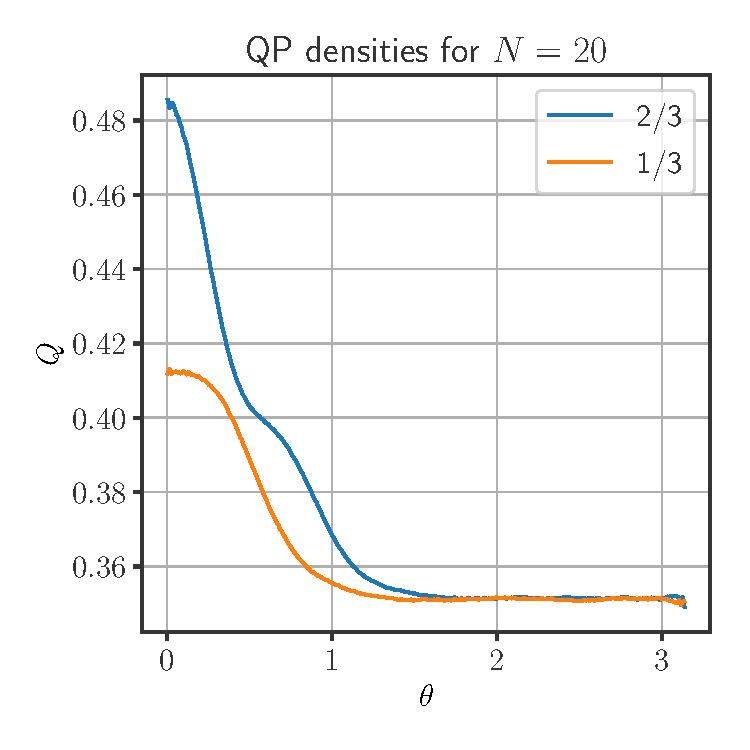
\includegraphics[width=2.5in]{figures/qp_densities_1b3_ansatz.pdf}
		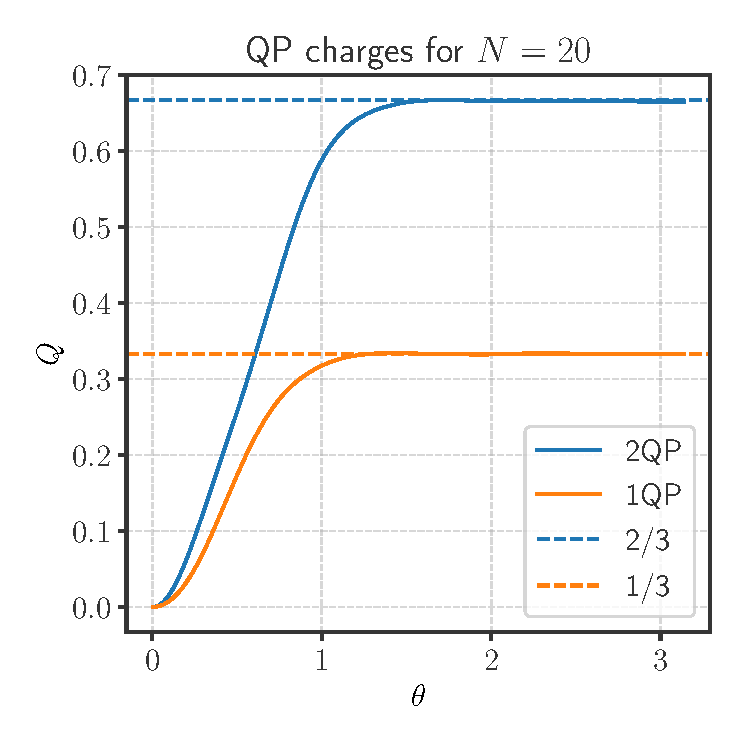
\includegraphics[width=2.5in]{figures/qp_charges_1b3_ansatz.pdf}
		\caption{Density $\rho$ and charge for $1/3$ $1$ and $2$ q-particles in a system of $N=20$}
	\end{figure}
	
	\subsection{Making ansatz numerics friendly}
	After establishing the proportionality, we wanted to check if we get $\nu=2/5$ ground state by completely filling $2^{nd}$ LL in our ansatz wf. But the problem arises because of derivatives $\partial_{u}, \partial_{u}$'s present in the $\hat{Y}^{Q-Q^{*}}_{Q^{*},n,m}$. They make the wf analytically intractible with each successive addtion of particle in highter LLs. Hence we wanted to check if we could drop the cross-terms in derivatives without losing important features of physics. This essentially means, replacing 
	
	\begin{align*}
		\partial_{u_i} &\rightarrow \sum_{k\neq i} \frac{2 v_k}{u_i v_k - u_k v_i} \\
		\partial_{v_i} &\rightarrow \sum_{k\neq i} \frac{2 u_k}{v_i u_k - v_k u_i} \\
 	\end{align*}
 	
 	and it allows us to write ansatz for higher LL very easily. Here is the overlap plot of \textit{full} ansatz with one when the cross-terms in the derivatives are ignored (for $2$ and $3$ qp's respectively).
 	
 	 \begin{figure}[h]
		\centering
		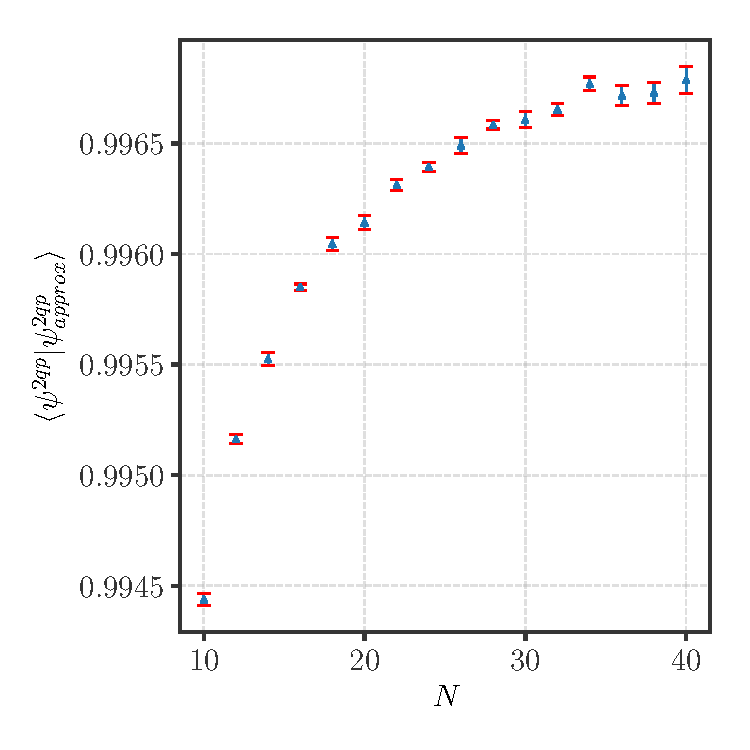
\includegraphics[width=2.5in]{figures/2QP_overlap_with_partcles.pdf}
		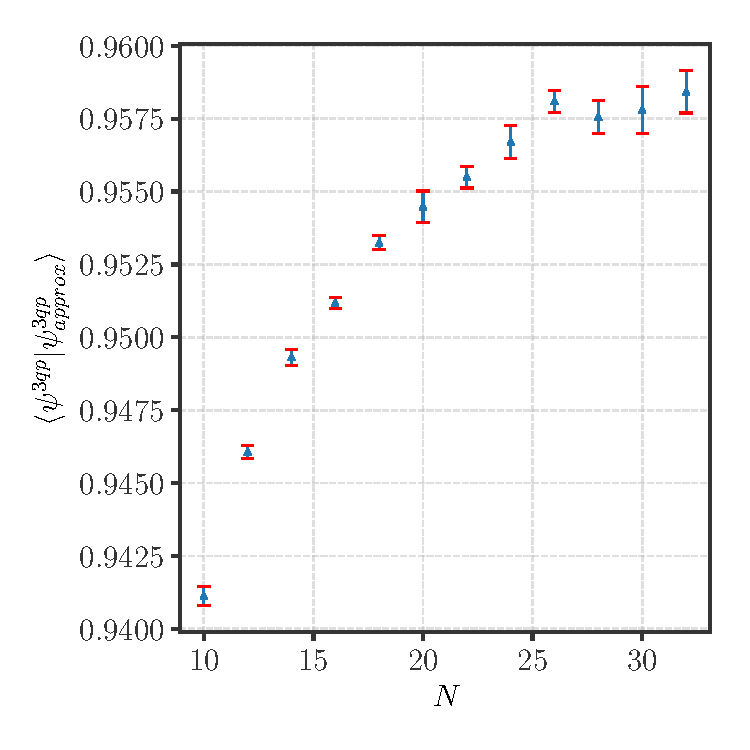
\includegraphics[width=2.5in]{figures/3QP_overlap_with_partcles.pdf}
		\caption{Overlaps of \textit{full} ansatz with modified one with $N$. Left $2$ qps and right is for $3$ qps}
	\end{figure}
	
	\pagebreak
	Finally, we have density and charge of $2/5$ quasi-hole, using the modified ansatz wf. 
	
	\begin{figure}[h]
		\centering
		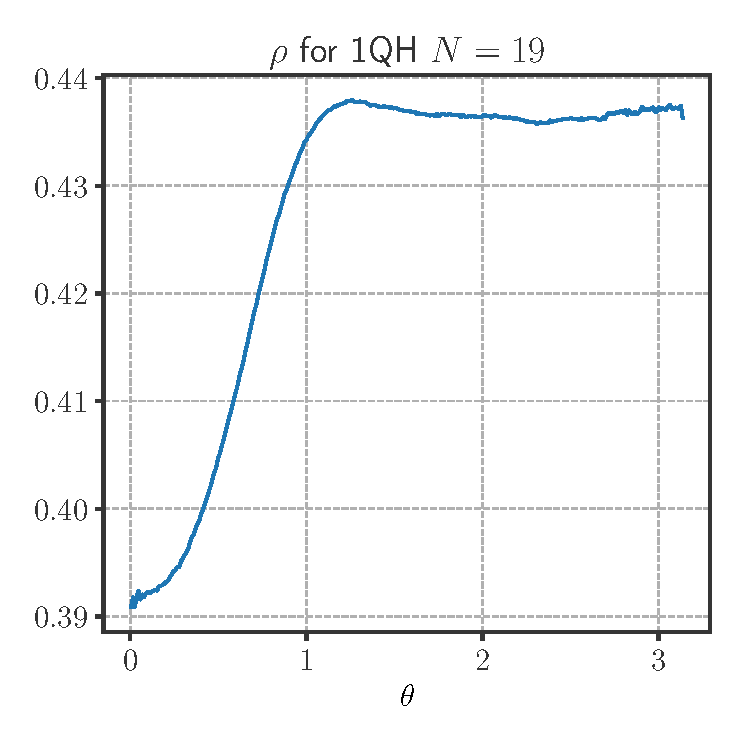
\includegraphics[width=2.5in]{figures/1qh_density_2b5_N19_ansatz.pdf}
		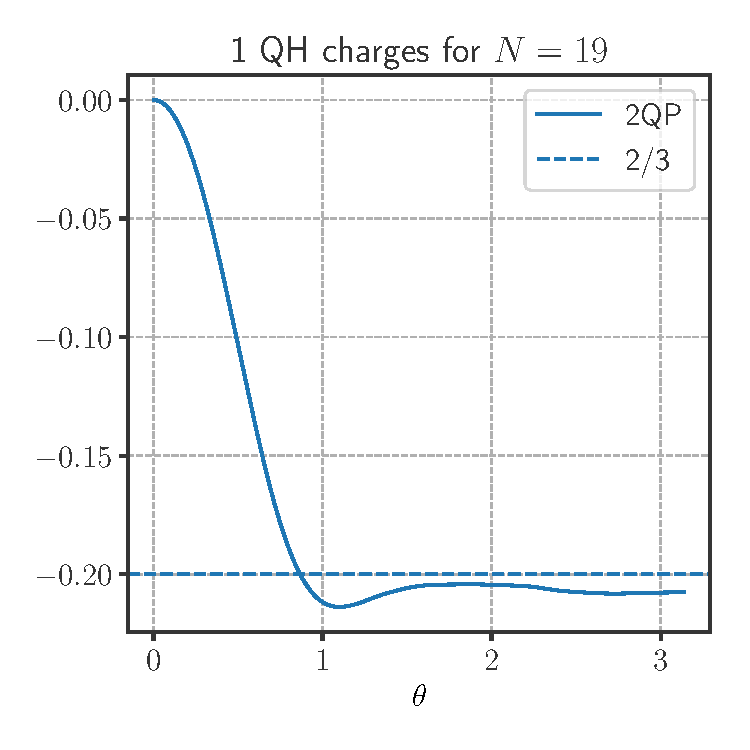
\includegraphics[width=2.5in]{figures/qh_charges_1b3_ansatz.pdf}
		\caption{Density and charge for $2/5$ q-hole using modified ansatz wf}
	\end{figure}
	
	\section{ToFix}
	
	\begin{enumerate}
		\item \todo Change the x-axis from $\theta$ to $\sqrt{Q}\theta$
		\item \done Fix ED density plots 
		\item \todo Compare $1/3$ $2$qp case for Full and approx wf 
		\item \todo Compare $1/3$ $1$qp case for ED and Full, different system sizes comparison
		\item \todo Compare densities of 1QH for ED, full and approx $2/5$ case
	\end{enumerate}
	
	\section{Todo}
	
	This is the list of calculations which are yet to be done :
	
	\begin{enumerate}
		\item overlap b/w ED and approximate $2/5$ state \\
		\item pair correlation function for $2/5$ ED and Approx state
	\end{enumerate}
	
	
\end{document}